%!TeX program = xelatex
\documentclass[12pt,a4paper,UTF8]{ctexart}
% 用户只提供了 main.tex 文本；实际 RUCReport.sty 尚未提供。
% 找到并审阅样式文件后可放到同目录；模板封面元信息按其定义填写。
\newif\ifRUCTemplate
\IfFileExists{RUCReport.sty}{\RUCTemplatetrue\usepackage{RUCReport}}{\RUCTemplatefalse}
\ifRUCTemplate\else
  \usepackage[margin=25mm,headheight=15pt]{geometry}
\fi
\usepackage{graphicx}
\usepackage{booktabs,longtable,tabularx,array}
\usepackage{xcolor,listings}
\usepackage{pdflscape}
\usepackage{placeins}
\usepackage{xurl}
\usepackage{hyperref}
\hypersetup{hidelinks,pdfauthor={KNOWVERSE 项目组},pdftitle={KNOWVERSE 项目报告写作框架}}
\urlstyle{same}
\renewcommand{\arraystretch}{1.22}
\setlength{\emergencystretch}{2em}
\setcounter{secnumdepth}{3}
\setcounter{tocdepth}{2}
\renewcommand{\thefigure}{\thesection-\arabic{figure}}
\renewcommand{\thetable}{\thesection-\arabic{table}}
\makeatletter
\@addtoreset{figure}{section}
\@addtoreset{table}{section}
\makeatother
\newcolumntype{Y}{>{\raggedright\arraybackslash}X}
\newcommand{\code}[1]{\texttt{\detokenize{#1}}}
\newcommand{\Writing}[2]{\par\smallskip\noindent\textbf{写作任务（#1）}：#2\par\smallskip}
\newcommand{\Evidence}[1]{\par\smallskip{\small\raggedright\noindent 证据入口：\path{#1}\par}}
\newcommand{\ChapterOwner}[2]{\noindent\textbf{主笔：#1；复核：#2。}\par\medskip}
\lstdefinestyle{SQL}{language=SQL,basicstyle=\small\ttfamily,breaklines=true,columns=fullflexible,
  numbers=left,numberstyle=\tiny\color{gray},numbersep=8pt,frame=single,
  keywordstyle=\bfseries\color{blue!50!black},showstringspaces=false,tabsize=2}

% 姓名、学号、最终版本与实际贡献由本人确认后填写，不代签。
\newcommand{\ProjectName}{知屿 KNOWVERSE}
\newcommand{\ProjectSubtitle}{基于学习记录与关系数据库的个人学习助手}
\newcommand{\ProjectTitle}{\ProjectName：\ProjectSubtitle}
\newcommand{\CourseName}{数据库系统概论}
\newcommand{\ReportDate}{2026 年 11 月 21 日}
\newcommand{\TeamInformation}{A：数据与身份；B：呈现与交互\\C：检索与智能；D：集成与交付\\姓名、学号、最终代码版本：待团队填写}

\begin{document}
\ifRUCTemplate
  \cover
\else
  \begin{titlepage}
  \centering
  \vspace*{18mm}
  {\zihao{2}\bfseries \CourseName\par}
  \vspace{22mm}
  {\zihao{1}\bfseries 项目报告写作框架\par}
  \vspace{14mm}
  {\zihao{3}\bfseries \ProjectName\par}
  \vspace{3mm}
  {\zihao{-3}\bfseries \ProjectSubtitle\par}
  \vspace{18mm}
  {\large \TeamInformation\par}
  \vfill
  {\large \ReportDate\par}
  \vspace{8mm}
  \begin{minipage}{.86\linewidth}\small
  本文件为报告架构、章节任务与协作分工预览，不是可直接提交的项目报告。
  当前使用基础封面；原模板样式文件补齐后再核对正式封面。
  \end{minipage}
  \end{titlepage}
\fi
\pagenumbering{Roman}
\section*{写作说明与协作分工}
\addcontentsline{toc}{section}{写作说明与协作分工}
课程要求报告包含需求分析、概要设计、详细设计和系统测试。数据库部分要有教材式 ER，讲清规范化与开发便利性的取舍，并审查大模型辅助设计的结果\cite{course}。
各人编辑自己负责的文件，写作提示用于查漏。可以调整小节顺序，选自己熟悉的例子，把图放在它要解释的段落旁。

\begin{table}[htbp]\centering\small
\begin{tabularx}{\linewidth}{lYY}
\toprule 成员角色 & 写在哪里 & 图放在哪里\\\midrule
A 数据库 & 数据库设计、成长与协作、模型辅助审查 & ER 与字段示例放建模，宽表分解放规范化，查询对照放查询设计\\
B 界面 & 需求分析、系统实现与交互 & 场景图放需求，真截图按操作顺序贯穿系统交互\\
C 答疑与检索 & 概要设计、答疑、历史与资料、记忆、摘要与总结 & 总架构图放概要设计，时序图和引用图放对应模块\\
D 测试与集成 & 判题、系统测试、部署与运行维护 & 判题图放练习，性能图放实验结果，部署图放迁移与启动\\\bottomrule
\end{tabularx}
\caption{各人负责的章节与配图}
\end{table}

各人把做过的事、作图源稿和运行证据一起交给 D。写正文时可以从一个操作讲起，把改动、理由和结果写具体。图注交代读者看到什么，真实截图注明实际操作与运行模式。

各人的章文件见 \path{docs/report/report-plan.md}。素材和此前的配图建议见 \path{docs/report/report-plan-detailed.md}。新图稿放 \path{assets/}。合稿后把本说明和各处提示换成正式正文。

\clearpage
\tableofcontents
\clearpage
\pagenumbering{arabic}
\section*{摘要}
\markboth{摘要}{摘要}
\addcontentsline{toc}{section}{摘要}
\Writing{C 起草，全员定稿}{正文完成后，简要说清学习记录管理遇到的问题、数据库怎样支撑核心功能、实验验证了什么。引用最终版本的实验结果。}
\noindent\textbf{关键词：}个人学习助手；关系数据库；关系建模；历史问答检索；数据完整性

\clearpage
\section{需求分析}\label{sec:requirements}
\ChapterOwner{B}{C}
\subsection{项目背景与目标}
\Writing{B}{解释历史问答难以整理、资料来源难追溯、练习与学习状态割裂的问题。给出可检验目标，说明系统管理学习事实，花园用于呈现。}
\subsection{用户角色与使用场景}
\Writing{B}{用一次学习过程说明需求。场景图放在这里，可以画从学生提问到回找原回答的操作，或用用例图概括角色与功能。}
\subsection{功能需求与优先级}
\Writing{B}{将答疑、时间/关键词/知识点历史检索列为课程必选，资料和训练列为推荐，成长与协作列为增强。每项给编号、输入、输出及验收条件。}
\subsection{数据需求与业务规则}
\Writing{B，A 核对}{从会话归属、引用具体片段、重复提交和撤销证据等实际例子里提炼规则，说清能观察到什么。}
\subsection{非功能需求}
\Writing{B}{持久化、隔离、并发一致性、失败恢复、可复现、移动端和可访问性。性能目标与实验结果分开，不把目标当成已达成。}
\subsection{需求追踪与系统范围}
\Writing{B，C 复核}{建立需求编号、实现模块和测试编号的对应表。说明 demo/live、班级 2D SVG、资料类型和生成题型的实际范围。}
\Evidence{docs/requirements-matrix.md; docs/features-explained.md}

\clearpage
\section{概要设计}\label{sec:architecture}
\ChapterOwner{C}{A、B}
\subsection{系统总体架构与边界}
\Writing{C，B 提供图}{画浏览器、页面/API、服务模块、数据访问层、PostgreSQL、外部模型、文件存储和独立 SQL 沙箱。箭头标请求或数据含义，模型不直接操作业务数据库。}
\subsection{模块职责与依赖}
\Writing{C}{按身份、问答、历史检索、资料、练习成长、班级协作分模块，说明责任和依赖，不只展示目录树。}
\subsection{主要数据流与信任边界}
\Writing{C，A 复核}{选一次答疑、一次作答画概要流程，标用户身份、外部调用、返回校验、短事务和落表位置。}
\subsection{技术选型与理由}
PostgreSQL 是本系统使用的关系数据库管理系统，负责保存、查询数据及执行约束和事务；16 表示主版本。报告的论证重点是关系如何设计、操作如何正确执行，版本号本身不作为创新点。
\Writing{C}{按真实工程说明 Next.js、TypeScript、Drizzle、模型接口的职责，实验章记录实际小版本和环境。}
\subsection{接口与异常约定}
\Writing{C}{选 5--8 个实际接口列方法、输入、输出、权限和失败处理，完整 API 放附录。接口名称从代码核对，不能按想象填写。}
\subsection{演示模式与真实模式}
\Writing{C}{说明 demo 不调用模型、live 使用外部服务；两者消息和证据持久化路径，以及出题和评分方式的差别。}
\Evidence{src/app/api/; src/server/; src/db/index.ts; docs/agent.md}

\clearpage
\section{数据库设计}\label{sec:database}
\ChapterOwner{A}{C、D}
\subsection{建模范围与数据域}
\Writing{A}{从业务事实划分身份、知识、学习世界、问答、资料、练习成长、协作、运维。区分概念模型、关系模式和物理设计。2026-11-17 目录快照有 55 个逻辑表、106 条 FK，排除分区子表和视图；定稿时重导并标实际日期。}

\subsection{教材式 ER 模型与语义}
主图精选核心学习链，包含 13 个实体、12 个菱形联系和 21 个椭圆属性。矩形为实体，菱形为联系，椭圆为属性，下划线标键，数字表示最大基数，双线表示全参与。图没有画出的字段通过核心列说明和分域字典补足。
\Writing{A}{逐段讲资料版本链、消息知识点链、作答证据链。说明消息角色 ISA 是同一消息表的分类；版本表采用全局 ID，不因有外键就认定为弱实体。主图与实现映射逐项核对。}
\begin{landscape}
\begin{figure}[p]\centering
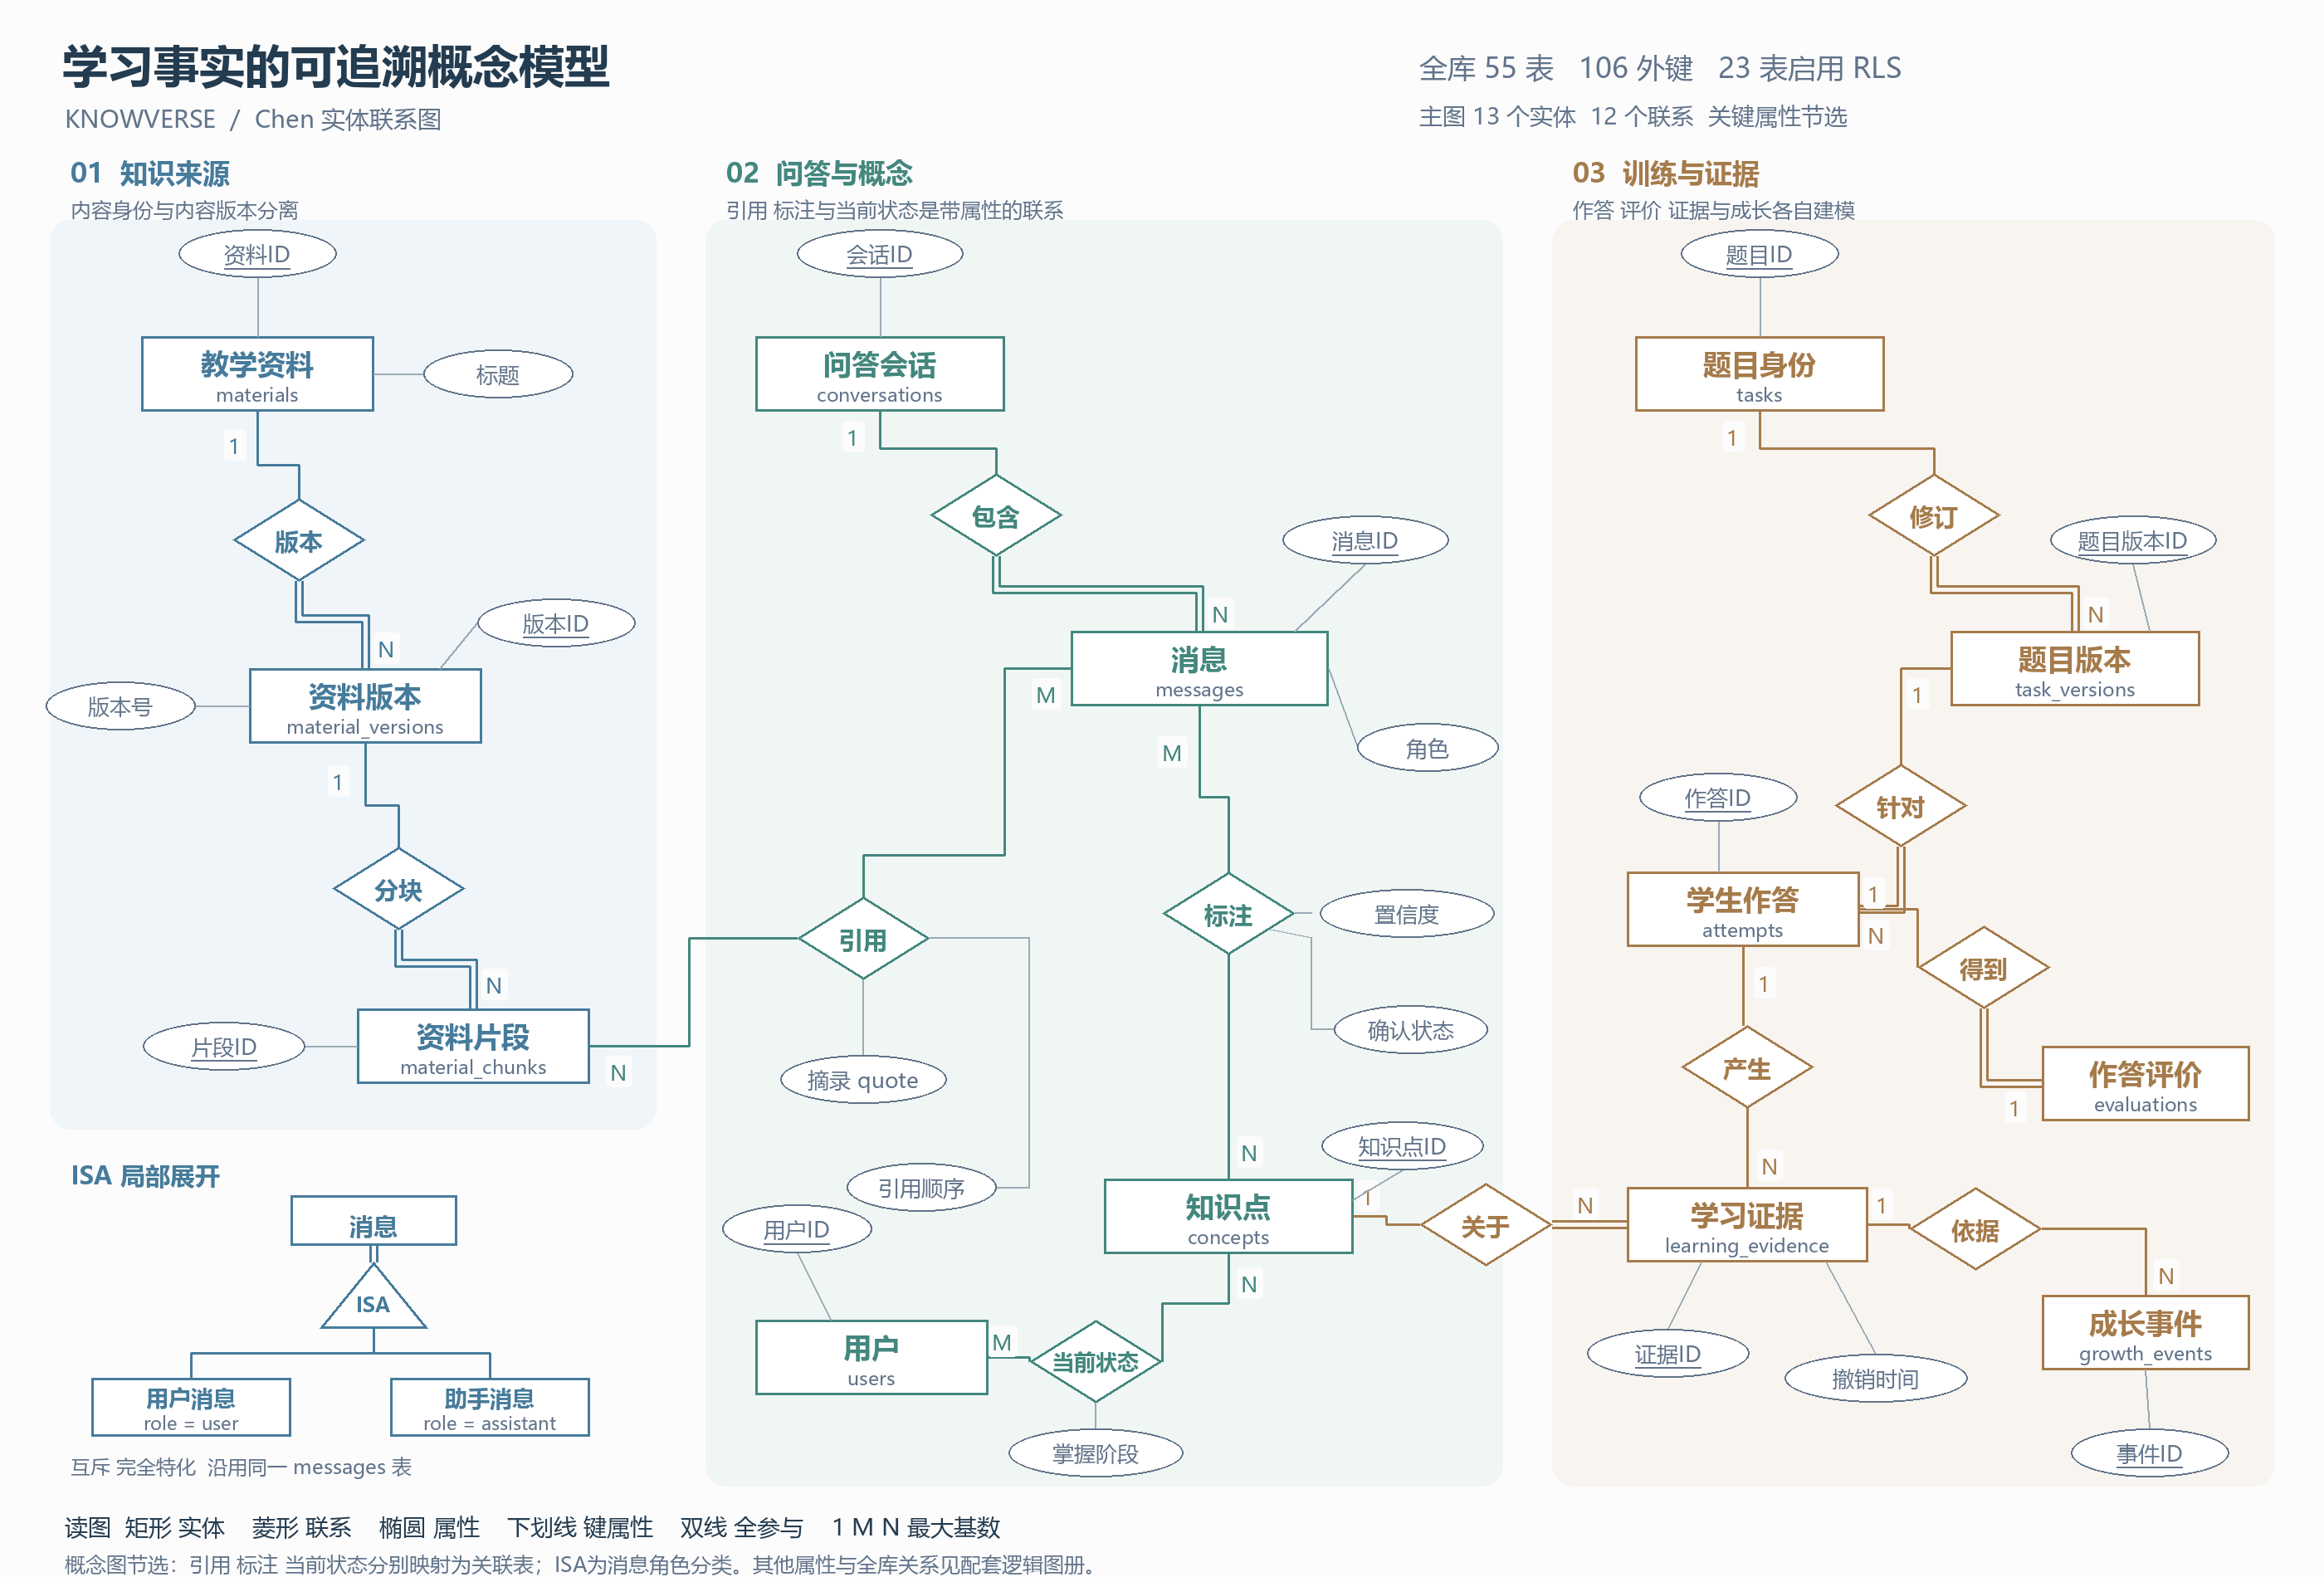
\includegraphics[width=\linewidth,height=.82\textheight,keepaspectratio]{../../er/advanced/03-learning-model.png}
\caption{实际系统核心 Chen 概念模型，属性经过精选；完整映射见图册}\label{fig:chen}
\end{figure}
\end{landscape}

\subsection{概念模型到关系模式的映射}
\Writing{A}{分别解释实体、1:N、M:N、带属性联系、自关联、ISA 如何映射。核心列至少覆盖问答标签、资料引用、练习证据三组，标类型、可空、PK/FK/UQ 和含义。}
\subsubsection{核心字段与示意数据}
以下列均来自系统目录，表中仅选关键列，非完整字典。C1、Q1、A2 等是方便讲解的符号，真实标识类型为 UUID，不能当作数据库实测记录。
\begin{table}[htbp]\centering\small
\begin{tabularx}{\linewidth}{lY}
\toprule 关系 & 精选字段及作用\\\midrule
\code{messages} & \code{id, conversation_id, user_id, seq, role, content, reply_to_id, status}：消息身份、归属、顺序、内容、回复对象与处理状态\\
\code{message_concepts} & \code{message_id, concept_id, source, status, confidence}：一条消息与一个知识点的关联及确认状态\\
\code{material_versions} & \code{id, material_id, version_no, status}：某份资料的确定版本\\
\code{material_chunks} & \code{id, version_id, ord, page_no, content}：该版本内的片段、位置与原文\\
\code{message_citations} & \code{id, message_id, chunk_id, ref_label, quote, ord}：一次回答引用哪个片段、摘录什么\\\bottomrule
\end{tabularx}
\caption{核心字段示意；类型、可空性与约束由作者补充完整}\label{tab:columns}
\end{table}
\Writing{A，C 核对}{补 Q1/A2 与片段 X1、版本 V1、资料 M1 的几行示意，展示按 chunk、version、material 外键追溯，再补作答/评价/证据/状态字段与实例。}

\subsection{候选键、函数依赖与规范化}
\subsubsection{候选键和函数依赖的业务含义}
\Writing{A}{先解释“哪些列能唯一确定一行”“某属性由谁决定”，再列 4--6 个真实关系的候选键与 FD。可空 UNIQUE、部分唯一、非最小超键单列；代理主键不代表其他依赖自动消失。}
\subsubsection{宽表异常、局部分解与无损连接}
\Writing{A}{把宽表和分解后的关系并排画在这里。用同一组用户、知识点和状态说明哪里重复、修改一条数据会影响哪些行，再给出局部无损分解的根据。}
\subsubsection{已核实结论与未证明边界}
\Writing{A，C 复核}{按最新范式复核分析版本、片段、知识点关联、引用、消息等。旧全库 46/5/4 统计已经撤回，不再宣称全库 BCNF、4NF、5NF。引用摘录由每次引用选择，不存在 \code{chunk_id} 决定 \code{quote} 的 FD。}

\subsection{受控冗余与应用便利性的权衡}
\code{messages.user_id} 与会话归属重复，对候选键 \code{(conversation_id,seq)} 存在部分依赖，严格不满足 2NF。系统保留它用于本表用户过滤，并用复合外键强制与会话一致。
\Writing{A}{再讲当前学习状态、倒排与汇总的维护、对账、读写代价。跨表可重算不是自动违反本表 3NF；少一次 JOIN 的预期不作为已经测得的收益。}

\subsection{完整性约束与业务规则}
\Writing{A}{用真实 DDL 说明 PK/FK/UNIQUE/NOT NULL/CHECK、复合与延迟约束。选引用、消息归属、本命花、先修防环、成员资格、幂等六例；解释约束、触发器、函数、应用检查各能覆盖什么。}

\subsection{查询语义与物理设计}\label{sec:query-design}
\subsubsection{用户要查什么、结果怎样组成}
\Writing{A，C 核对}{用一组问答说明关键词、时间、知识点与排序。知识点查询返回问题及其最新回答：Q1 最新 A2，旧 A1 有 K、Q1/A2 无 K，则筛 K 不能返回 Q1；问题与最新回答都命中也只出一组。}
\subsubsection{原查询与候选集合改写}
\Writing{A}{把原查询和候选集合改写并排画在这里，标出筛标签、取最新回答和去重。两侧用同一组示例行。讲清结果为什么相同，再贴必要的 SQL。实验结果放第\ref{sec:testing}章。}
\subsubsection{索引与维护成本}
\Writing{A}{把 B 树、GIN/倒排、部分索引与实际读写对应。用执行计划说明扫描次数变化，保留覆盖索引负优化案例，不泛称加索引必然更快。}

\subsection{事务、并发与失败恢复}
\Writing{A}{模型调用放事务外；前后短事务保存 pending 与回答引用。作答结算解释锁、唯一性和幂等，评价/证据/状态/事件/outbox 原子写入。并发重复提交、最后名额、中途失败各一例；outbox 原子写入不等于消费可靠性已闭环。}

\subsection{数据库安全与访问控制}
\Writing{A}{owner、\code{kv_app}、\code{kv_sandbox} 分开；事务局部身份与 RLS；甲乙用户、无上下文、池复用用非所有者验证；班级共享按成员与偏好受控。23 表 RLS 是快照覆盖信息，不代表全部表同策略或绝对安全。}

\subsection{视图、时态、审计与模式演进}
\Writing{A}{视图/物化/增量的新鲜度、审计分区、有效证据重放、迁移演进与从零建立。CDC、在线 DDL、批处理等专项择要写，详材放附录。}
\Evidence{docs/er/advanced/; docs/schema/normalization-analysis.md; docs/schema/candidate-keys.md; src/db/schema.ts; drizzle/}

\clearpage
\section{核心业务详细设计}\label{sec:detailed}
\ChapterOwner{各模块负责人，C 统筹}{A、D 交叉复核}
各节按用户目标、输入与前置条件、步骤、读写表、事务边界、输出、异常和权限、完整实例组织。关系定义引用第\ref{sec:database}章，测试结果引用第\ref{sec:testing}章。
\subsection{个性化答疑与上下文组织}
\Writing{C}{用一条真实问答讲上下文、检索、生成、校验和保存。时序图放在本节，用浏览器、服务、模型和数据库几条泳道画清请求先后，标出事务和失败重试。}
\subsection{历史检索、定位与继续提问}
\Writing{C}{组合关键词、时间、知识点、学科，解释用户时区、最新回答、分页、高亮、定位窗口和续问。用一组问题 ID 展示结果缩小；查询设计引用\ref{sec:query-design}节，不重写性能表。}
\Evidence{src/server/chat.ts; src/server/history.ts; src/server/agent/; tests/history.test.ts}

\subsection{资料整理、版本与引用核验}
\Writing{C}{提取正文/备注、位置、分块、版本和候选概念。画“检索器产生候选片段→模型选择编号和摘录→后端核对编号、正文标记、原文连续摘录→合法引用入库”。解释谁决定引用、谁提出知识点、谁确认。引用摘录合法不等于整句结论被证明。给片段经版本找到资料的存取实例。}
\Evidence{src/server/materials.ts; src/server/retrieval/; tests/materials-collab.test.ts; tests/citation-fd.test.ts}

\subsection{薄弱点练习、评价与 SQL 沙箱}
\Writing{D}{交选题/生成/评价/结算流程。区分题库按薄弱点选题、live 模型生成变式、选择数值规则、SQL 执行比较、开放题 live/demo 评分。说明独立数据库、只读事务、超时、语句限制、NULL/重复行/排序/浮点容差。附合法等价和非法查询实例、读写表与错误反馈。}
\Evidence{src/server/practice.ts; src/server/sandbox.ts; sandbox/; docs/sql/sandbox.md; tests/sandbox.test.ts}

\subsection{学习证据、当前状态与成长}
\Writing{A}{评价、证据、当前状态、成长事件是不同事实。交规则表、一次结算/撤销/重算实例，解释提示与独立作答区别、来源、撤销时间、时间轴，阶段不是模型随意判定。}
\subsection{班级分享、共学与知识卡}
\Writing{A}{成员资格、分享偏好、互补匹配依据、并发名额、贡献、卡片版本与发布。图形星系为 2D SVG；共享范围不等于开放全部学习数据。}
\Evidence{src/server/growth.ts; src/server/classes.ts; tests/practice-growth.test.ts; tests/galaxy-view.test.ts}

\subsection{已实现的记忆管理与用户控制}
\Writing{C，控制篇幅}{来源消息、事实/偏好、纠正链、失效时间、禁用/删除、会话摘要。讲明现有实现和控制规则，不把记忆保存写成模型理解的证明，不加入尚未实施的向量检索成果。}
\Evidence{docs/memory.md; tests/memory.test.ts; drizzle/0030_rag_tables.sql}


\clearpage
\section{系统实现与交互}\label{sec:implementation}
\ChapterOwner{B}{C、D}
\subsection{工程组织与实现环境}
\Writing{B}{主要目录、职责、锁定版本与构建方式，不抄全部依赖。}
\subsection{真实用户操作实例}
\Writing{B}{沿提问、查看来源、组合检索、回原会话、作答、查看成长依据，选 6--8 张真截图。每图写日期、操作/输入/输出、相关表、demo/live/预置。以下仅为现有运行材料接入示例，应按最终版本更新。}
\begin{figure}[htbp]\centering
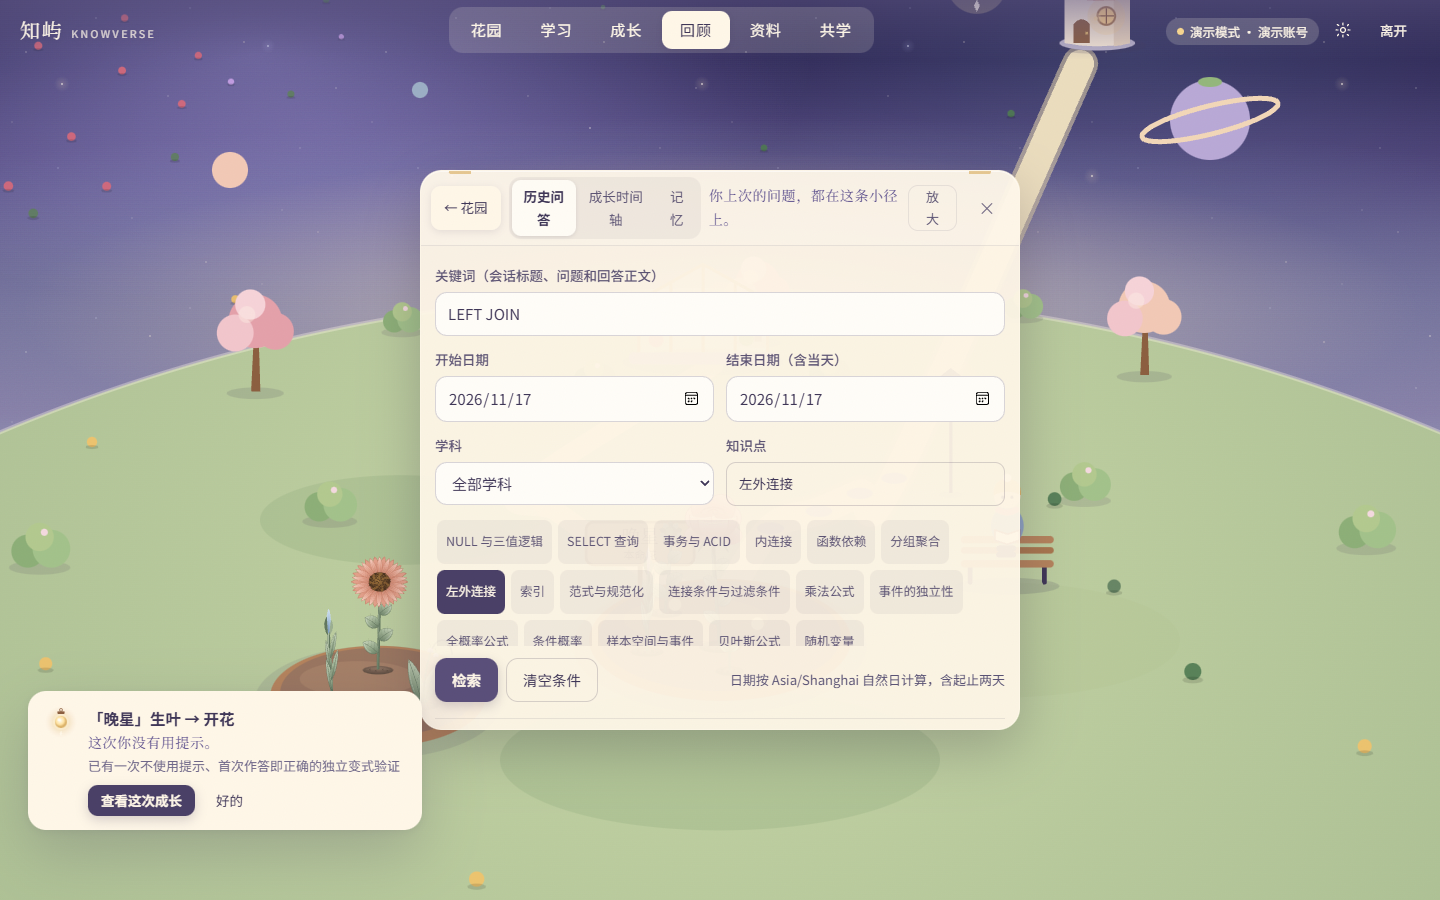
\includegraphics[width=.93\linewidth]{../../screenshots/acceptance-2026-11-17/09-history-combined.png}
\caption{2026-11-17 真实浏览器验收截图：组合历史检索；demo 模式、静态绘本降级}\label{fig:history-shot}
\end{figure}
\FloatBarrier
\subsection{数据库状态到界面的映射}
\Writing{B，A 核对}{概念与植物、学习状态与阶段、证据与成长说明怎样映射。数据事实驱动界面，不能倒写为动画驱动结算。}
\subsection{异常处理与反馈}
\Writing{B}{等待、模型失败、资料不足、引用不通过、无结果、重复提交、沙箱不可用等状态和实际反馈。}
\subsection{响应式、可访问性与降级}
\Writing{B}{移动、键盘、低动效、无 WebGL；班级为 2D SVG，主花园与降级另述。软件渲染截图不推导真机帧率。}
\subsection{实现难点与取舍}
\Writing{B}{选 2--3 个真实问题讲原因、修改、回归与剩余限制。HTML 动画只是流程示意，不替代真实截图或性能记录。}
\Evidence{docs/screenshots/acceptance-2026-11-17/; docs/screenshots/ui/; docs/visual-redesign.md}

\clearpage
\section{系统测试与实验评测}\label{sec:testing}
\ChapterOwner{D 汇总，A/B/C 各交专项}{A、C}
\subsection{测试策略、环境与数据}
\Writing{D}{单元、真实 PG 服务、HTTP、浏览器、性能专项分层，日期、代码版本、角色、模式与数据规模写全。2026-11-17 的全量基线是 250 例/37 文件，封稿必须复测最终代码；本框架编译不等于应用复测。}
\subsection{功能与业务异常测试}
\Writing{C/B/D}{按需求编号给输入、操作、预期、实际和记录路径，覆盖答疑、组合检索、版本引用、练习、重试、证据修正。}
\subsection{完整性、事务与并发测试}
\Writing{A 提供，D 汇总}{错误外键/归属、并发幂等、最后名额、中途回滚、状态对账，提供前后行数和失败原因，不能只写通过。}
\subsection{权限与沙箱安全测试}
\Writing{A/D}{\code{kv_app} 双用户、无上下文、连接复用、非法写入、SQL 沙箱安全与等价。说明测试覆盖边界，不声称全面安全。}
\subsection{历史查询优化实验}
\Writing{A 主笔，C 核对语义，D 复现}{先解释冷门/热门是知识点命中数据量，不是缓存状态。原/改写在同 4 万消息、两用户、相同条件/权限下返回完整行、顺序和总数一致，再比较 P50/P95/吞吐/扫描。}
\begin{table}[htbp]\centering\small
\begin{tabular}{llrr}\toprule
知识点命中量 & 并发 & 原查询 P95/ms & 改写 P95/ms\\\midrule
少（冷门） & 1 & 78.74 & 4.66\\
少（冷门） & 4 & 142.15 & 5.15\\
多（热门） & 1 & 144.00 & 134.32\\
多（热门） & 4 & 273.33 & 103.82\\\bottomrule
\end{tabular}
\caption{2026-11-17 历史实验，\code{kv_app}、每组 20 请求、预热 2 次；非本次复测}\label{tab:history-bench}
\end{table}
\FloatBarrier
\Writing{A 提数据，D 作图}{紧接结果表放分组对照图，完整展示应用角色下不同命中量、不同并发的原查询与改写 P95，标毫秒和样本。解释已验证的结果等价、测量范围与限制。}
\subsection{来源与检索质量专项}
\Writing{C}{区分检索命中、摘录合法、语义正确。已有集 50 问是 40 有资料+10 无资料，38/40 为有效引用，不是答案准确率；8 主题改写不当 50 独立主题。人工金标准缺失如实写，记忆指标同样具体定义。}
\subsection{端到端与界面验收}
\Writing{B/D}{列日期、浏览器、视口、WebGL。2026-11-17 的 15/15 主流程为静态降级，不能扩大成 3D 全流程；引用真实截图与结果 JSON。}
\subsection{缺陷修复与测试局限}
\Writing{D，收各模块材料}{挑有证据的缺陷写清现象、定位、修改和复测。有必要时放诊断截图或前后结果表。报告中的汇总数字从相应版本的原始输出核对。}
\Evidence{docs/test-report.md; docs/test-evidence/vitest-history-2026-11-17.json; docs/sql/history-optimization.json; docs/sql/rag-c4-closeout.md}

\clearpage
\section{部署与运行维护}
\ChapterOwner{D}{A}
\subsection{运行环境与配置}
\Writing{D}{说明 Node/PG、依赖锁、环境变量职责、owner/应用/沙箱连接，报告不含真实密钥。}
\subsection{从零建立与迁移}
\Writing{D，A 核对}{把本地建库、迁移、种子数据、应用启动和验收画成一张步骤图放在这里。用一次干净环境运行的输出说明实际走到了哪一步，并交代已有数据库怎样向前迁移。}
\subsection{测试环境、基准与 CI}
\Writing{D}{\code{knowverse_test} 与 \code{knowverse_bench} 隔离，CI 步骤与实际运行分开。YAML 存在不等于远程通过。}
\subsection{维护、备份与故障恢复}
\Writing{D}{分区、统计对账、pending、outbox/积压；备份与恢复标明步骤示例或真实演练、恢复点与数据损失边界。}
\subsection{最终版本与交付包}
\Writing{D}{核对最终 commit/tag、运行说明、演示账号、PDF/TeX/资源、已知限制。保护规则、Release 和外部部署按实际记录。}
\Evidence{README.md; docs/release.md; .github/workflows/ci.yml; tests/global-setup.ts}

\clearpage
\section{大模型辅助设计与审查}\label{sec:llm-review}
\ChapterOwner{A 汇总，每人提交实际案例}{全员}
\subsection{使用范围与记录方法}
\Writing{A}{列模型参与工作、输入、原始证据和事后整理的边界。旧文档模型名/日期/初始表数须成员核实，不伪造聊天、会议或人工签认。}
\subsection{初始候选与设计迭代}
\Writing{A}{选 3--5 个真实变化，展示候选、问题、改动和最终实现。历史 45 表与当前 55 表属于不同版本。}
\subsection{采纳与调整的合理性}
\Writing{A，各交一例}{版本拆分、M:N、复合 FK、幂等等，逐项分析语义、键、FD、约束和开发便利性，不只写模型建议合理。}
\subsection{否决、反例与纠错}
\Writing{A/C/D}{展示已撤回范式统计、错误引用 FD、覆盖索引负优化等真实案例，用合法反例或执行计划解释纠错。}
\subsection{人工审阅与责任边界}
\Writing{全员本人填写}{每人至少一例，记录姓名、时间、方法、结论、修改、证据及另一人的复核。未审阅不得代填通过或代签。}
\subsection{辅助效果与局限}
\Writing{A}{总结帮助与必须理解、验证之处。代码生成量不等于数据库设计质量；无法追溯的记录明确说明。}
\Evidence{docs/llm-assisted-design.md; docs/schema/normalization-analysis.md; docs/sql/index-decisions.md}

\clearpage
\section{总结、局限与后续计划}
\ChapterOwner{C 汇总}{全员}
\subsection{完成情况与主要工作}
\Writing{C}{逐项回应课程必选与推荐需求，概括关系建模、版本溯源、事务幂等、隔离、查询实测。功能依据来自实际代码与证据\cite{project}。}
\subsection{当前局限}
\Writing{全员}{全库 FD 未逐项证明、规模/设备测试有限、答案语义金标准不足、outbox/恢复演练不足、2D 班级星系等，按最终状态核对。}
\subsection{后续任务与验收}
\Writing{C 汇总}{优先写来源归属审查、更多偏斜/HTTP 实验、人工来源支持性标注、备份恢复、消费监控。逐项列问题、动作、验收；尚未实施的技术不写成成果。}

\clearpage
\phantomsection
\addcontentsline{toc}{section}{参考文献}
\bibliographystyle{unsrt}
\bibliography{reference}
\clearpage
\appendix
\section{数据库目录与图册}
\Writing{A}{给完整表目录、核心字典、高清图索引、统计日期和排除对象，主文不贴不可读的 55 表缩略图。}
\Evidence{docs/er/advanced/README.md; docs/er/advanced/schema-metadata.json; docs/schema/data-dictionary.md}
\section{核心 SQL 与约束}
\Writing{A/C}{收录引用追溯、历史筛选、状态和班级统计、重要约束，标实际文件/函数与版本。正文只保留分析必需片段。}
\Evidence{docs/sql/core_queries.sql; src/server/history.ts; drizzle/}
\section{测试与实验记录索引}
\Writing{D 汇总}{每项列命令、环境、日期、代码版本、数据规模、原始结果和复现说明，失败与限制保留。}
\Evidence{docs/test-evidence/; docs/qa-checklist.md; docs/sql/history-optimization.json}
\section{接口、截图与离线演示}
\Writing{C/B}{索引真实 API、运行截图、离线阶段 HTML。动画标示意，不把网页动画当实测运行；资料用相对路径打包。}
\Evidence{src/app/api/; docs/screenshots/; docs/briefings/}

\clearpage
\section{成员贡献与审阅记录}
\Writing{D 维护，全员实填}{建议分工见写作说明，下面记录实际完成的工作。姓名、学号、贡献比例和签认必须本人确认；计划不直接转换为贡献比例。}
\begin{longtable}{p{.12\linewidth}p{.20\linewidth}p{.28\linewidth}p{.25\linewidth}}
\toprule 角色 & 姓名、学号 & 实际工作与交付 & PR/commit/证据、复核\\\midrule
\endhead
A & 待本人填写 & 待按实际填写 & 待交证据与复核\\
B & 待本人填写 & 待按实际填写 & 待交证据与复核\\
C & 待本人填写 & 待按实际填写 & 待交证据与复核\\
D & 待本人填写 & 待按实际填写 & 待交证据与复核\\\bottomrule
\end{longtable}
\Writing{全员}{每人第 8 章审查案例另列日期、对象、核对方法、结论、修改和证据；最终统一确认事实与引用版本。}

\end{document}
